\documentclass[pdftex,11pt,openany]{book}\usepackage[]{graphicx}\usepackage[]{color}
%% maxwidth is the original width if it is less than linewidth
%% otherwise use linewidth (to make sure the graphics do not exceed the margin)
\makeatletter
\def\maxwidth{ %
  \ifdim\Gin@nat@width>\linewidth
    \linewidth
  \else
    \Gin@nat@width
  \fi
}
\makeatother

\definecolor{fgcolor}{rgb}{0.345, 0.345, 0.345}
\newcommand{\hlnum}[1]{\textcolor[rgb]{0.686,0.059,0.569}{#1}}%
\newcommand{\hlstr}[1]{\textcolor[rgb]{0.192,0.494,0.8}{#1}}%
\newcommand{\hlcom}[1]{\textcolor[rgb]{0.678,0.584,0.686}{\textit{#1}}}%
\newcommand{\hlopt}[1]{\textcolor[rgb]{0,0,0}{#1}}%
\newcommand{\hlstd}[1]{\textcolor[rgb]{0.345,0.345,0.345}{#1}}%
\newcommand{\hlkwa}[1]{\textcolor[rgb]{0.161,0.373,0.58}{\textbf{#1}}}%
\newcommand{\hlkwb}[1]{\textcolor[rgb]{0.69,0.353,0.396}{#1}}%
\newcommand{\hlkwc}[1]{\textcolor[rgb]{0.333,0.667,0.333}{#1}}%
\newcommand{\hlkwd}[1]{\textcolor[rgb]{0.737,0.353,0.396}{\textbf{#1}}}%

\usepackage{framed}
\makeatletter
\newenvironment{kframe}{%
 \def\at@end@of@kframe{}%
 \ifinner\ifhmode%
  \def\at@end@of@kframe{\end{minipage}}%
  \begin{minipage}{\columnwidth}%
 \fi\fi%
 \def\FrameCommand##1{\hskip\@totalleftmargin \hskip-\fboxsep
 \colorbox{shadecolor}{##1}\hskip-\fboxsep
     % There is no \\@totalrightmargin, so:
     \hskip-\linewidth \hskip-\@totalleftmargin \hskip\columnwidth}%
 \MakeFramed {\advance\hsize-\width
   \@totalleftmargin\z@ \linewidth\hsize
   \@setminipage}}%
 {\par\unskip\endMakeFramed%
 \at@end@of@kframe}
\makeatother

\definecolor{shadecolor}{rgb}{.97, .97, .97}
\definecolor{messagecolor}{rgb}{0, 0, 0}
\definecolor{warningcolor}{rgb}{1, 0, 1}
\definecolor{errorcolor}{rgb}{1, 0, 0}
\newenvironment{knitrout}{}{} % an empty environment to be redefined in TeX

\usepackage{alltt}

%\documentclass[11pt,openany]{book}

% команды АК.
\newcommand{\calL}{\mathcal{L}}
\newcommand{\bs}[1]{\boldsymbol{#1}} 
\newcommand{\hypo}{\mathcal{H}} 
\newcommand{\simhypo}{\ensuremath{\mathrel{\stackrel{\hypo_0}{\sim}}}}

%%%%%%%%%%%%%%%%%%%%%%%  Загрузка пакетов  %%%%%%%%%%%%%%%%%%%%%%%%%%%%%%%%%%
% кусок от урсса
%\usepackage[60x90,headers,11pt]{format}

%\textheight=494pt%
%\textwidth=322pt%
%
%\oddsidemargin=0pt%
%\evensidemargin=0pt
%\topmargin=-1pt \headsep=14pt \headheight=22pt \voffset=-28pt
%\hoffset=-50pt


\clubpenalty=10000  
\widowpenalty=10000

%\overfullrule=5pt
%\hfuzz=1.5mm 
%\baselineskip=12pt plus 0.18pt minus 0.1pt


\pagestyle{headings}
% конец куска от урсса




% специальная версия для knitr'а. Исключает graphicx

%\usepackage{showkeys} % показывать метки в готовом pdf 

\usepackage{etex} % расширение классического tex
% в частности позволяет подгружать гораздо больше пакетов, чем мы и займёмся далее

%\usepackage{mathtext} % русские буквы в формулах? (и без неё работает)
% Например, $x_{\text{один}}$

%\usepackage{cmap} % для поиска русских слов в pdf --- теперь работает без этого
% а с cmap не работает печать на принтер ;)
\usepackage{verbatim} % для многострочных комментариев
\usepackage{makeidx} % для создания предметных указателей
\usepackage[X2,T2A]{fontenc}
\usepackage[utf8]{inputenc} % задание utf8 кодировки исходного tex файла
\usepackage{setspace}
\usepackage{amsmath,amsfonts,amssymb,amsthm}
\usepackage{mathrsfs} % sudo yum install texlive-rsfs
\usepackage{dsfont} % sudo yum install texlive-doublestroke
\usepackage{array,multicol,multirow,bigstrut} % sudo yum install texlive-multirow
\usepackage{indentfirst} % установка отступа в первом абзаце главы
\usepackage[russian]{babel} % выбор языка для документа
\usepackage{bm}
\usepackage{bbm} % шрифт с двойными буквами
%\usepackage[perpage]{footmisc}

\usepackage{dcolumn} % центрирование по разделителю для apsrtable

% создание гиперссылок в pdf
\usepackage[pdftex,unicode,colorlinks=true,urlcolor=blue,hyperindex,breaklinks]{hyperref} 

% свешиваем пунктуацию 
% теперь знаки пунктуации могут вылезать за правую границу текста, при этом текст выглядит ровнее
\usepackage{microtype}

\usepackage{textcomp}  % Чтобы в формулах можно было русские буквы писать через \text{}

% размер листа бумаги
\usepackage[paperwidth=145mm,paperheight=215mm,
height=182mm,width=113mm,top=20mm,includefoot]{geometry}
%\usepackage[paper=a4paper,top=13.5mm, bottom=13.5mm,left=16.5mm,right=13.5mm,includefoot]{geometry}

\usepackage{xcolor}

% \usepackage[pdftex]{graphicx} % для вставки графики, убрано, т.к. knitr похоже сам добавляет

\usepackage{float,longtable}
\usepackage{soulutf8}

\usepackage{enumitem} % дополнительные плюшки для списков
%  например \begin{enumerate}[resume] позволяет продолжить нумерацию в новом списке

\usepackage{mathtools}
\usepackage{cancel,xspace} % sudo yum install texlive-cancel

% \usepackage{minted} % display program code with syntax highlighting
% требует установки pygments и python 

\usepackage{numprint} % sudo yum install texlive-numprint
\npthousandsep{,}\npthousandthpartsep{}\npdecimalsign{.}

\usepackage{embedfile} % Чтобы код LaTeXа включился как приложение в PDF-файл

\usepackage{subfigure} % для создания нескольких рисунков внутри одного

\usepackage{tikz,pgfplots} % язык для рисования графики из latex'a
\usetikzlibrary{trees} % tikz-прибамбас для рисовки деревьев
\usepackage{tikz-qtree} % альтернативный tikz-прибамбас для рисовки деревьев
\usetikzlibrary{arrows} % tikz-прибамбас для рисовки стрелочек подлиннее

\usepackage{todonotes} % для вставки в документ заметок о том, что осталось сделать
% \todo{Здесь надо коэффициенты исправить}
% \missingfigure{Здесь будет Последний день Помпеи}
% \listoftodos --- печатает все поставленные \todo'шки


% более красивые таблицы
\usepackage{booktabs}
% заповеди из докупентации: 
% 1. Не используйте вертикальные линни
% 2. Не используйте двойные линии
% 3. Единицы измерения - в шапку таблицы
% 4. Не сокращайте .1 вместо 0.1
% 5. Повторяющееся значение повторяйте, а не говорите "то же"



%\usepackage{asymptote} % пакет для рисовки графики, должен идти после graphics
% но мы переходим на tikz :)

%\usepackage{sagetex} % для интеграции с Sage (вероятно тоже должен идти после graphics)

% metapost создает упрощенные eps файлы, которые можно напрямую включать в pdf 
% эта группа команд декларирует, что файлы будут этого упрощенного формата
% если metapost не используется, то этот блок не нужен
\usepackage{ifpdf} % для определения, запускается ли pdflatex или просто латех
\ifpdf
	\DeclareGraphicsRule{*}{mps}{*}{}
\fi
%%%%%%%%%%%%%%%%%%%%%%%%%%%%%%%%%%%%%%%%%%%%%%%%%%%%%%%%%%%%%%%%%%%%%%


%%%%%%%%%%%%%%%%%%%%%%%  Внедрение tex исходников в pdf файл  %%%%%%%%%%%%%%%%%%%%%%%%%%%%%%%%%%
\embedfile[desc={Main tex file}]{\jobname.tex} % Включение кода в выходной файл
\embedfile[desc={title_bor}]{title_bor_utf8_knitr.tex}

%%%%%%%%%%%%%%%%%%%%%%%%%%%%%%%%%%%%%%%%%%%%%%%%%%%%%%%%%%%%%%%%%%%%%%



%%%%%%%%%%%%%%%%%%%%%%%  ПАРАМЕТРЫ  %%%%%%%%%%%%%%%%%%%%%%%%%%%%%%%%%%
\setstretch{1}                          % Межстрочный интервал
\flushbottom                            % Эта команда заставляет LaTeX чуть растягивать строки, чтобы получить идеально прямоугольную страницу
\righthyphenmin=2                       % Разрешение переноса двух и более символов
%\pagestyle{plain}                       % Нумерация страниц снизу по центру.
%\widowpenalty=300                     % Небольшое наказание за вдовствующую строку (одна строка абзаца на этой странице, остальное --- на следующей)
%\clubpenalty=3000                     % Приличное наказание за сиротствующую строку (омерзительно висящая одинокая строка в начале страницы)
\setlength{\parindent}{1.5em}           % Красная строка.
%\captiondelim{. }
\setlength{\topsep}{0pt}
%%%%%%%%%%%%%%%%%%%%%%%%%%%%%%%%%%%%%%%%%%%%%%%%%%%%%%%%%%%%%%%%%%%%%%



%%%%%%%% Это окружение, которое выравнивает по центру без отступа, как у простого center
\newenvironment{center*}{%
  \setlength\topsep{0pt}
  \setlength\parskip{0pt}
  \begin{center}
}{%
  \end{center}
}
%%%%%%%%%%%%%%%%%%%%%%%%%%%%%%%%%%%%%%%%%%%%%%%%%%%%%%%%%%%%%%%%%%%%%%


%%%%%%%%%%%%%%%%%%%%%%%%%%% Правила переноса  слов
\hyphenation{ }
%%%%%%%%%%%%%%%%%%%%%%%%%%%%%%%%%%%%%%%%%%%%%%%%%%%%%%%%%%%%%%%%%%%%%%

\emergencystretch=2em


% DEFS
\def \mbf{\mathbf}
\def \msf{\mathsf}
\def \mbb{\mathbb}
\def \tbf{\textbf}
\def \tsf{\textsf}
\def \ttt{\texttt}
\def \tbb{\textbb}

\def \wh{\widehat}
\def \wt{\widetilde}
\def \ni{\noindent}
\def \ol{\overline}
\def \cd{\cdot}
\def \fr{\frac}
%\def \bs{\backslash}
\def \lims{\limits}
\DeclareMathOperator{\dist}{dist}
\DeclareMathOperator{\VC}{VCdim}
\DeclareMathOperator{\card}{card}
\DeclareMathOperator{\sign}{sign}
\DeclareMathOperator{\sgn}{sign}
\DeclareMathOperator{\Tr}{\mbf{Tr}}
\DeclareMathOperator{\tr}{tr}


\def \xfs{(x_1,\ldots,x_{n-1})}
\DeclareMathOperator*{\argmin}{arg\,min}
\DeclareMathOperator*{\amn}{arg\,min}
\DeclareMathOperator*{\amx}{arg\,max}
\DeclareMathOperator{\trace}{tr}
\DeclareMathOperator{\rk}{rk}


\DeclareMathOperator{\Corr}{Corr}
\DeclareMathOperator{\sCorr}{sCorr}
\DeclareMathOperator{\sCov}{sCov}
\DeclareMathOperator{\sVar}{sVar}

\DeclareMathOperator{\Cov}{Cov}
\DeclareMathOperator{\Var}{Var}
\DeclareMathOperator{\corr}{Corr}
\DeclareMathOperator{\cov}{Cov}
\DeclareMathOperator{\var}{Var}
\DeclareMathOperator{\bin}{Bin}
\DeclareMathOperator{\Bin}{Bin}
\DeclareMathOperator{\rang}{rang}
\DeclareMathOperator*{\plim}{plim}
\DeclareMathOperator{\MSE}{MSE}

\providecommand{\iff}{\Leftrightarrow}
\providecommand{\hence}{\Rightarrow}

\def \ti{\tilde}
\def \wti{\widetilde}

\def \mA{\mathcal{A}}
\def \mB{\mathcal{B}}
\def \mC{\mathcal{C}}
\def \mE{\mathcal{E}}
\def \mF{\mathcal{F}}
\def \mH{\mathcal{H}}
\def \mL{\mathcal{L}}
\def \mN{\mathcal{N}}
\def \mU{\mathcal{U}}
\def \mV{\mathcal{V}}
\def \mW{\mathcal{W}}


\def \R{\mbb R}
\def \N{\mbb N}
\def \Z{\mbb Z}
\def \P{\mbb{P}}
\def \p{\mbb{P}}
\newcommand{\E}{\mathbb{E}}
\def \D{\msf{D}}
\def \I{\mbf{I}}

\def \QQ{\mbb Q}
\def \RR{\mbb R}
\def \NN{\mbb N}
\def \ZZ{\mbb Z}
\def \PP{\mbb P}


\def \a{\alpha}
\def \b{\beta}
\def \t{\tau}
\def \dt{\delta}
\newcommand{\e}{\varepsilon}
\def \ga{\gamma}
\def \kp{\varkappa}
\def \la{\lambda}
\def \sg{\sigma}
\def \sgm{\sigma}
\def \tt{\theta}
\def \ve{\varepsilon}
\def \Dt{\Delta}
\def \La{\Lambda}
\def \Sgm{\Sigma}
\def \Sg{\Sigma}
\def \Tt{\Theta}
\def \Om{\Omega}
\def \om{\omega}

%\newcommand{\p}{\partial}

\def \ni{\noindent}
\def \lq{\glqq}
\def \rq{\grqq}
\def \lbr{\linebreak}
\def \vsi{\vspace{0.1cm}}
\def \vsii{\vspace{0.2cm}}
\def \vsiii{\vspace{0.3cm}}
\def \vsiv{\vspace{0.4cm}}
\def \vsv{\vspace{0.5cm}}
\def \vsvi{\vspace{0.6cm}}
\def \vsvii{\vspace{0.7cm}}
\def \vsviii{\vspace{0.8cm}}
\def \vsix{\vspace{0.9cm}}
\def \VSI{\vspace{1cm}}
\def \VSII{\vspace{2cm}}
\def \VSIII{\vspace{3cm}}

\newcommand{\bls}[1]{\boldsymbol{#1}}
\newcommand{\bsA}{\boldsymbol{A}}
\newcommand{\bsH}{\boldsymbol{H}}
\newcommand{\bsI}{\boldsymbol{I}}
\newcommand{\bsP}{\boldsymbol{P}}
\newcommand{\bsR}{\boldsymbol{R}}
\newcommand{\bsS}{\boldsymbol{S}}
\newcommand{\bsX}{\boldsymbol{X}}
\newcommand{\bsY}{\boldsymbol{Y}}
\newcommand{\bsZ}{\boldsymbol{Z}}
\newcommand{\bse}{\boldsymbol{e}}
\newcommand{\bsq}{\boldsymbol{q}}
\newcommand{\bsy}{\boldsymbol{y}}
\newcommand{\bsbeta}{\boldsymbol{\beta}}
\newcommand{\fish}{\mathrm{F}}
\newcommand{\Fish}{\mathrm{F}}
\renewcommand{\phi}{\varphi}
\newcommand{\ind}{\mathds{1}}
\newcommand{\inds}[1]{\mathds{1}_{\{#1\}}}
\renewcommand{\to}{\rightarrow}
\newcommand{\sumin}{\sum\limits_{i=1}^n}
\newcommand{\ofbr}[1]{\bigl( \{ #1 \} \bigr)}     % Например, вероятность события. Большие круглые, нормальные фигурные скобки вокруг аргумента
\newcommand{\Ofbr}[1]{\Bigl( \bigl\{ #1 \bigr\} \Bigr)} % Например, вероятность события. Больше больших круглые, большие фигурные скобки вокруг аргумента
\newcommand{\oeq}{{}\textcircled{\raisebox{-0.4pt}{{}={}}}{}} % Равно в кружке
\newcommand{\og}{\textcircled{\raisebox{-0.4pt}{>}}}  % Знак больше в кружке

% вместо горизонтальной делаем косую черточку в нестрогих неравенствах
\renewcommand{\le}{\leqslant}
\renewcommand{\ge}{\geqslant}
\renewcommand{\leq}{\leqslant}
\renewcommand{\geq}{\geqslant}


\newcommand{\figb}[1]{\bigl\{ #1  \bigr\}} % большие фигурные скобки вокруг аргумента
\newcommand{\figB}[1]{\Bigl\{ #1  \Bigr\}} % Больше больших фигурные скобки вокруг аргумента
\newcommand{\parb}[1]{\bigl( #1  \bigr)}   % большие скобки вокруг аргумента
\newcommand{\parB}[1]{\Bigl( #1  \Bigr)}   % Больше больших круглые скобки вокруг аргумента
\newcommand{\parbb}[1]{\biggl( #1  \biggr)} % большие-большие круглые скобки вокруг аргумента
\newcommand{\br}[1]{\left( #1  \right)}    % круглые скобки, подгоняемые по размеру аргумента
\newcommand{\fbr}[1]{\left\{ #1  \right\}} % фигурные скобки, подгоняемые по размеру аргумента
\newcommand{\eqdef}{\mathrel{\stackrel{\rm def}=}} % знак равно по определению
\newcommand{\const}{\mathrm{const}}        % const прямым начертанием
\newcommand{\zdt}[1]{\textit{#1}}
\newcommand{\ENG}[1]{\foreignlanguage{british}{#1}}
\newcommand{\ENGs}{\selectlanguage{british}}
\newcommand{\RUSs}{\selectlanguage{russian}}
\newcommand{\iid}{\text{i.\hspace{1pt}i.\hspace{1pt}d.}}

\newdimen\theoremskip
\theoremskip=0pt
\newenvironment{note}{\par\vskip\theoremskip\textbf{Замечание.\xspace}}{\par\vskip\theoremskip}
\newenvironment{hint}{\par\vskip\theoremskip\textbf{Подсказка.\xspace}}{\par\vskip\theoremskip}
\newenvironment{ist}{\par\vskip\theoremskip Источник:\xspace}{\par\vskip\theoremskip}

\newcommand*{\tabvrulel}[1]{\multicolumn{1}{|c}{#1}}
\newcommand*{\tabvruler}[1]{\multicolumn{1}{c|}{#1}}

\newcommand{\II}{{\fontencoding{X2}\selectfont\CYRII}}   % I десятеричное (английская i неуместна)
\newcommand{\ii}{{\fontencoding{X2}\selectfont\cyrii}}   % i десятеричное
\newcommand{\EE}{{\fontencoding{X2}\selectfont\CYRYAT}}  % ЯТЬ
\newcommand{\ee}{{\fontencoding{X2}\selectfont\cyryat}}  % ять
\newcommand{\FF}{{\fontencoding{X2}\selectfont\CYROTLD}} % ФИТА
\newcommand{\ff}{{\fontencoding{X2}\selectfont\cyrotld}} % фита
\newcommand{\YY}{{\fontencoding{X2}\selectfont\CYRIZH}}  % ИЖИЦА
\newcommand{\yy}{{\fontencoding{X2}\selectfont\cyrizh}}  % ижица

%%%%%%%%%%%%%%%%%%%%% Определение разрядки разреженного текста и задание красивых многоточий
\sodef\so{}{.15em}{1em plus1em}{.3em plus.05em minus.05em}
\newcommand{\ldotst}{\so{...}}
\newcommand{\ldotsq}{\so{?\hbox{\hspace{-0.61ex}}..}}
\newcommand{\ldotse}{\so{!..}}
%%%%%%%%%%%%%%%%%%%%%%%%%%%%%%%%%%%%%%%%%%%%%%%%%%%%%%%%%%%%%%%%%%%%%%

%%%%%%%%%%%%%%%%%%%%%%%%%%%%% Команда для переноса символов бинарных операций
\def\hm#1{#1\nobreak\discretionary{}{\hbox{$#1$}}{}}
%%%%%%%%%%%%%%%%%%%%%%%%%%%%%%%%%%%%%%%%%%%%%%%%%%%%%%%%%%%%%%%%%%%%%%

%\setlist[enumerate,1]{label=\arabic*., ref=\arabic*, partopsep=0pt plus 2pt, topsep=0pt plus 1.5pt,itemsep=0pt plus .5pt,parsep=0pt plus .5pt}
%\setlist[itemize,1]{partopsep=0pt plus 2pt, topsep=0pt plus 1.5pt,itemsep=0pt plus .5pt,parsep=0pt plus .5pt}

% Эти парни затем, если вдруг не захочется управлять списками из-под уютненького enumitem
% или если будет жизненно важно, чтобы в списках были именно русские буквы.
%\setlength{\partopsep}{0pt plus 3pt}
%\setlength{\topsep}{0pt plus 2pt}
%\setlength{\itemsep}{0 plus 1pt}
%\setlength{\parsep}{0 plus 1pt}

%на всякий случай пока есть
%теоремы без нумерации и имени
%\newtheorem*{theor}{Теорема}

%"Определения","Замечания"
%и "Гипотезы" не нумеруются
%\newtheorem*{defin}{Определение}
%\newtheorem*{rem}{Замечание}
%\newtheorem*{conj}{Гипотеза}

%"Теоремы" и "Леммы" нумеруются
%по главам и согласованно м/у собой
%\newtheorem{theorem}{Теорема}
%\newtheorem{lemma}[theorem]{Лемма}

% Утверждения нумеруются по главам
% независимо от Лемм и Теорем
%\newtheorem{prop}{Утверждение}
%\newtheorem{cor}{Следствие} 


% чисто эконометрические сокращения:

\def \useR{$[$R$]$ }

%% эконометрические сокращения
\def \hb{\hat{\beta}}
\def \hs{\hat{s}}
\def \hy{\hat{y}}
\def \hY{\hat{Y}}
\def \he{\hat{\varepsilon}}
\def \v1{\vec{1}}
\def \e{\varepsilon}
\def \hVar{\widehat{\Var}}
\def \hCorr{\widehat{\Corr}}
\def \hCov{\widehat{\Cov}}

%% алая и белая розы
%% запускается так: \WhiteRose[масштаб], например, \WhiteRose[0.5]
\newcommand{\WhiteRose}[1]{\begingroup
\setbox0=\hbox{
\includegraphics[scale=#1]{/home/boris/science/econometrix/em301/roses/Yorkshire_rose.pdf}}%
\parbox{\wd0}{\box0}\endgroup}

\newcommand{\RedRose}[1]{\begingroup
\setbox0=\hbox{
\includegraphics[scale=#1]{/home/boris/science/econometrix/em301/roses/Lancashire_rose.pdf}}%
\parbox{\wd0}{\box0}\endgroup}

\newcommand{\WhiteRoseLine}{
\begin{center}
\WhiteRose{0.3} Версия Белой Розы \WhiteRose{0.3}
\end{center}}

\newcommand{\RedRoseLine}{
\begin{center}
\RedRose{0.3} Версия Алой Розы \RedRose{0.3}
\end{center}}




% стандартизация
% эпсилон во временных рядах --- белый шум, а в остальных сюжетах --- остатки, подумать
% транспонирование --- штрих

% задачи типа "воспроизведите тест такой-то ручками в R" -> в тему согласно тесту, а не в доп. задачи по программированию

% идеи задач:
% * Задача на корреляционную матрицу по реальным данным require(quantmod)
% Задача про суеверную Мырли. Можно ли там что-то про se сказать?
% теорему FWL в массы!
% симуляционные задачи на ошибки 1, 2 рода, мощность
% E_t(X) или с указанием сигма-алгебры

% выложить преамбулу


% перегнанные банки:
% 1 ---20

% осталось:
% задача 12, компьютерное про пи (алгоритмы вычисления)
% распределить проверить наличие программистко-сюжетных упражнений


% для отдельной упаковки решений
%%%% версия с ОКРУЖЕНИЯМИ вместо комманд

% специальная штука под задачник
% создает команды:
% \problem{ текст задачи }
% \solution{ текст решения }
% \problemonly  - после этой команды будут печататься только \problem{} и \problemtext{}
% \solutiononly - после этой команды будут печататься только \solution{} и \solutiontext{}
% \problemandsolution - после этой команды печатается все
% \secsolution - задает новую (виртуальную) секцию для решений

% может потребоваться %\addtocounter{secsolution}{число глав без задач решений, не прогнанных через problemonly}

% как работать
% файл с решениями отдельной главы должен выглядеть так:
% \problem{ dddd} \solution{ddddddd}
% \problem{df sldk} \solution{ dfssd}

% главный файл может выглядеть двумя способами:

% Способ 1. (для решений контрольной, рядом задачи и ответы)
% \problemandsolution
% \input{file with problems}

% Способ 2. (для задачника, сначала все задачи, затем все ответы)
% \problemonly
% \input{file with problems}

% \solutiononly
% \input{file with problems}

% ААААААААААААААААААААААА надо делать!!!!
% Способ 3. - основной (вариант способа 2)

% \problemonly2
% \input{file with problems}

%\solutiononly - эта команда сама сделает все!




% файл с задачами:
% \section{Первая}
% \problem{ dddd} \solution{ddddddd}
% \problem{df sldk} \solution{ dfssd}
% \problemtext{Этот текст не будет напечатан после solutiononly}
% \section{Вторая}
% \problem{ ааа} \solution{dыва}
% \problem{ыавыв} \solution{ ыва}
% \solutiontext{Этот текст не будет напечатан после problemonly}



% начало кода:

\let\oldchapter\chapter % сохраняем команду \chapter, т.к. мы ее переопределим
\let\oldsection\section % сохраняем команду \section, т.к. мы ее переопределим

\newcommand{\restorechapter}{ % команда для восстановления \section \subsection
\renewcommand{\section}[1]{\oldsection{##1}}
\renewcommand{\chapter}[1]{\oldchapter{##1}}
}

\newcounter{problem}[chapter]
%создаем новый счетчик "problem", 
% будет автоматом сбрасываться на 0 при старте нового раздела
% при создании счетчик сам встанет на 0

\newcounter{secsolution}
% - это номер секции решаемой задачи (поскольку решения идут в одной секции, то номер секции надо менять в ручную)
\newcounter{solution}[secsolution]
% - это номер решаемой задачи, сам сбрасывается при увеличении secsolution на 1



\renewcommand{\thesecsolution}{\arabic{secsolution}}
% команда \thesecsolution просто выводит номер secsolution

\newcommand{\newsecsolution}{
\stepcounter{secsolution} % без создания ссылки увеличит secsolution на 1 со сбросом подчиненного счетчика
}
% команда \newsecsolution увеличит номер секции на 1 и установит номер решения внутри секции равным 0

\renewcommand{\theproblem}{\thechapter.\arabic{problem}.}
\renewcommand{\thesolution}{\thesecsolution.\arabic{solution}.}
% обновляем команду \theproblem - она должна выводить номер секции и номер задачи внутри секции
% почему обновляем? - потому, что она создалась при создании счетчика problem

% \newcommand{\problem}[1]{}
\newenvironment{problem}{%
  \catcode`\{=12
  \catcode`\}=12
  \DoNullproblem
}{%
  \ignorespacesafterend
}


\begingroup
  \catcode`\(=1
  \catcode`\)=2
  \catcode`\{=12
  \catcode`\}=12
  \def\x(%
    \endgroup
    \newcommand\DoNullproblem()
    \long\def\DoNullproblem##1\end{problem}(\end(problem))
  )
\x




%\newcommand{\solution}[1]{}
\newenvironment{solution}{%
  \catcode`\{=12
  \catcode`\}=12
  \DoNullsolution
}{%
  \ignorespacesafterend
}


\begingroup
  \catcode`\(=1
  \catcode`\)=2
  \catcode`\{=12
  \catcode`\}=12
  \def\x(%
    \endgroup
    \newcommand\DoNullsolution()
    \long\def\DoNullsolution##1\end{solution}(\end(solution))
  )
\x

% создаем команды \problem, \solution с одним аргументом, которые ничего не делает
% ниже они будут переопределены



\newenvironment{problemtext}{%
  \catcode`\{=12
  \catcode`\}=12
  \DoNullproblemtext
}{%
  \ignorespacesafterend
}


\begingroup
  \catcode`\(=1
  \catcode`\)=2
  \catcode`\{=12
  \catcode`\}=12
  \def\x(%
    \endgroup
    \newcommand\DoNullproblemtext()
    \long\def\DoNullproblemtext##1\end{problemtext}(\end(problemtext))
  )
\x


\newenvironment{solutiontext}{%
  \catcode`\{=12
  \catcode`\}=12
  \DoNullsolutiontext
}{%
  \ignorespacesafterend
}


\begingroup
  \catcode`\(=1
  \catcode`\)=2
  \catcode`\{=12
  \catcode`\}=12
  \def\x(%
    \endgroup
    \newcommand\DoNullsolutiontext()
    \long\def\DoNullsolutiontext##1\end{solutiontext}(\end(solutiontext))
  )
\x

% эти две команды будут выводить текст, заложенный внутри них только внутри соответствующей секции, в другой - ничего не будет делать
% в отличие от этой команды \problem \solution делают ссылки, слово "задача" и пр.


\newcommand{\problemonly}{
% эта команда переопределяет команду \problem и другие. Нам нужно печатать только условия.

% ставим на 0 все счетчики
\setcounter{problem}{0}
\setcounter{solution}{0}
\setcounter{secsolution}{0}


% команда \problemtext печатает то, что ей передают в качестве аргумента
% команда \solutiontext игнорируется
\renewenvironment{problemtext}{}{}

\renewenvironment{solutiontext}{%
  \catcode`\{=12
  \catcode`\}=12
  \DoNullsolutiontext
}{%
  \ignorespacesafterend
}

% теперь команда \section помимо своих стандартных функций еще и увеличит secsolution на 1.
\renewcommand{\chapter}[1]{\oldchapter{##1}\newsecsolution}
\renewcommand{\section}[1]{\oldsection{##1}}
% \subsection - стандартная


\renewenvironment{problem}{%
\refstepcounter{problem}
% \phantomsection % создаем точку привязки для команды \label % не нужна, т.к. есть refstepcounter
\textbf{Задача} 
\hyperref[s\theproblem]{\theproblem} % гиперссылка на метку "s1.1."
\label{p\theproblem} % метка "p1.1." 
\par
}{}


%\renewcommand{\solution}[1]{}
\renewenvironment{solution}{%
  \catcode`\{=12
  \catcode`\}=12
  \DoNullsolution
}{%
  \ignorespacesafterend
}



}

\newcommand{\solutiononly}{
% эта команда переопределяет команду \solution

\setcounter{problem}{0}
\setcounter{solution}{0}
\setcounter{secsolution}{0}

\renewenvironment{problemtext}{%
  \catcode`\{=12
  \catcode`\}=12
  \DoNullproblemtext
}{%
  \ignorespacesafterend
}

\renewenvironment{solution}{}{}

\renewcommand{\chapter}[1]{\newsecsolution} % можно сюда чего-то добавить, чтобы решения отделялись как-то по секциям
\renewcommand{\section}[1]{}

\renewenvironment{problem}{%
  \catcode`\{=12
  \catcode`\}=12
  \DoNullproblem
}{%
  \ignorespacesafterend
}

\renewenvironment{solution}{%
\refstepcounter{solution}
% \phantomsection
\hyperref[p\thesolution]{\thesolution} \label{s\thesolution}
}{}

} % end of definition for \solutiononly

\newcommand{\problemandsolution}{
% эта команда переопределяет команды \solution, \problem

\setcounter{problem}{0}
\setcounter{solution}{0}
\setcounter{secsolution}{0}

\renewcommand{\problemtext}[1]{##1}
\renewcommand{\solutiontext}[1]{##1}

\renewcommand{\chapter}[1]{\oldchapter{##1}\newsecsolution}
\renewcommand{\section}[1]{\oldsection{##1}}

\renewcommand{\problem}[1]{
\refstepcounter{problem}
% \phantomsection % создаем точку привязки для команды \label
\textbf{Задача} 
\hyperref[s\theproblem]{\theproblem} % гиперссылка на метку "s1.1."
\label{p\theproblem} % метка "p1.1." 
\par ##1}
\renewcommand{\solution}[1]{
\refstepcounter{solution}
% \phantomsection
\hyperref[p\thesolution]{\thesolution} \label{s\thesolution}
##1}
}





\title{Эконометрика \\ {\small с Монте-Карло и эконометрессами} \\ в задачах и упражнениях}
\author{Дмитрий Борзых, Борис Демешев}
\date{\today}

\makeindex % команда для создания предметного указателя
\bibliographystyle{plain} % стиль оформления ссылок
\IfFileExists{upquote.sty}{\usepackage{upquote}}{}


\begin{document}







%\listoftodos

% МНК


\problemonly




\chapter{Гетероскедастичность}


\begin{problem}
Что такое гетероскедастичность? Гомоскедастичность?
\end{problem}
\begin{solution}
\end{solution}

\begin{problem}
В модели $y=\hb_1+\hb_2 x+\e$ присутствует гетероскедастичность вида $\Var(\e_i)=\sigma^2 x^2_i$. Как надо преобразовать исходные регрессоры и зависимую переменную, чтобы устранить гетероскедастичность? 
\end{problem}

\begin{solution}
Поделить зависимую переменную и каждый регрессор, включая единичный столбец, на $|x_i|$.
\end{solution}


\begin{problem}
В модели $y=\hb_1+\hb_2 x+\e$ присутствует гетероскедастичность вида $\Var(\e_i)=\lambda |x_i|$. Как надо преобразовать исходные регрессоры и зависимую переменную, чтобы устранить гетероскедастичность? 
\end{problem}

\begin{solution}
Поделить зависимую переменную и каждый регрессор, включая единичный столбец, на $\sqrt{|x_i|}$.
\end{solution}


\begin{problem}
Известно, что после деления каждого уравнения регрессии $y_i = \beta_1 + \beta_2 x_i + \e_i$ на $x_i^2$ гетероскедастичность ошибок была устранена. Какой вид имела дисперсия ошибок, $\Var(\e_i)$?
\end{problem}

\begin{solution}
$\Var(\e_i)=cx_i^4$
\end{solution}


\begin{problem}
Известно, что после деления каждого уравнения регрессии $y_i = \beta_1 + \beta_2 x_i + \e_i$ на $\sqrt{x_i}$ гетероскедастичность ошибок была устранена. Какой вид имела дисперсия ошибок, $\Var(\e_i)$?
\end{problem}
\begin{solution}
$\Var(\e_i)=c x_i$
\end{solution}


\begin{problem}
Диаграмма рассеяния стоимости квартиры в Москве (в 1000\$) и общей площади квартиры имеет вид:

\begin{knitrout}
\definecolor{shadecolor}{rgb}{0.969, 0.969, 0.969}\color{fgcolor}\begin{kframe}
\begin{alltt}
\hlkwd{ggplot}\hlstd{(flats,}\hlkwd{aes}\hlstd{(}\hlkwc{x}\hlstd{=totsp,}\hlkwc{y}\hlstd{=price))}\hlopt{+}\hlkwd{geom_point}\hlstd{()}\hlopt{+}
    \hlkwd{labs}\hlstd{(}\hlkwc{x}\hlstd{=}\hlstr{"Общая площадь, кв. м."}\hlstd{,}
    \hlkwc{y}\hlstd{=}\hlstr{"Цена квартиры, 1000$"}\hlstd{)}
\end{alltt}
\end{kframe}
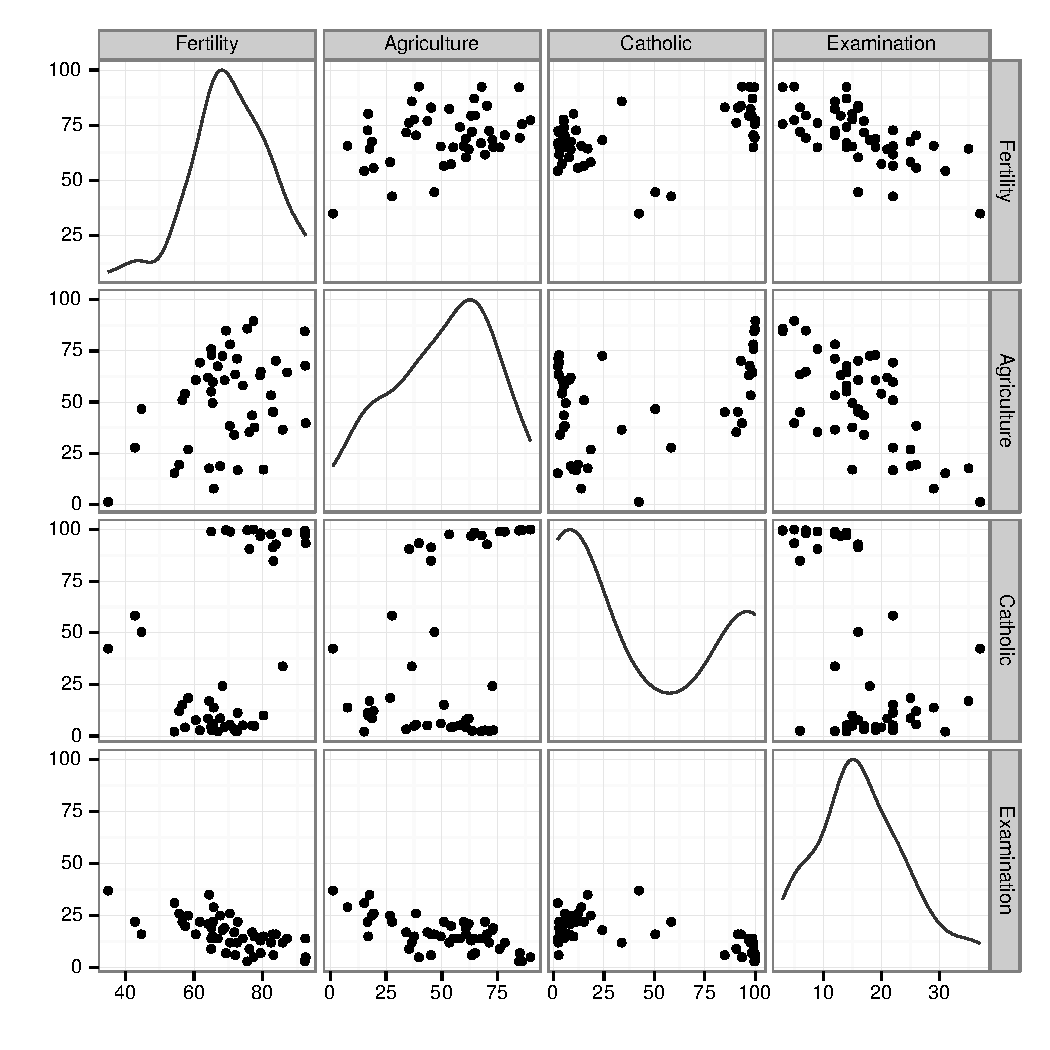
\includegraphics[width=7cm,height=7cm]{figure/unnamed-chunk-2} 

\end{knitrout}


Какие подходы к оцениванию зависимости имеет смысл посоветовать исходя из данного графика?
\end{problem}


\begin{solution}
По графику видно, что с увеличением общей площади увеличивается разброс цены. Поэтому разумно, например, рассмотреть следующие подходы:
\begin{enumerate}
\item Перейти к логарифмам, т.е. оценивать модель $\ln price_i=\beta_1+\beta_2 \ln totsp_i +\varepsilon_i$
\item Оценивать квантильную регрессию. В ней угловые коэффициенты линейной зависимости будут отличаться для разных квантилей переменной $price$.
\item Обычную модель линейной регрессии с гетероскедастичностью вида $Var(\varepsilon_i)=\sigma^2 totsp_i^2$
\end{enumerate} 
\end{solution}



\begin{problem}
По наблюдениям $x=(1,2,3)'$, $y=(2,-1,3)'$ оценивается модель $y=\b_1+\b_2 x+\e$. Ошибки $\e$ гетероскедастичны и известно, что $\Var(\e_i)=\sigma^2 \cdot x_i^2$. 
\begin{enumerate}
\item Найдите оценки $\hb_{ols}$ с помощью МНК и их ковариационную матрицу
\item Найдите оценки $\hb_{gls}$ с помощью обобщенного МНК и их ковариационную матрицу 
\end{enumerate}  
\end{problem}

\begin{solution}
\end{solution}




\begin{problem}
Для линейной регрессии $y_i = \beta_1 + \beta_2 x_i + \beta_3 z_i + \e_i$ была
выполнена сортировка наблюдений по возрастанию переменной $x$. Исходная модель оценивалась по разным частям выборки:

\begin{tabular}{c|cccc}
Выборка & $\hb_1$ & $\hb_2$ & $\hb_3$ & $RSS$ \\
\hline 
$i=1,\ldots, 30$ & $1.21$ & $1.89$ & $2.74$ & $48.69$ \\ 
$i=1,\ldots, 11$ & $1.39$ & $2.27$ & $2.36$ & $10.28$ \\ 
$i=12,\ldots, 19$ & $0.75$ & $2.23$ & $3.19$ & $5.31$ \\ 
$i=20,\ldots, 30$ & $1.56$ & $1.06$ & $2.29$ & $14.51$ \\ 
\end{tabular} 

Известно, что ошибки в модели являются независимыми нормальными случайными величинами с нулевым математическим ожиданием. Протестируйте
ошибки на гетероскедастичность на уровне значимости 5\%.
\end{problem}


\begin{solution}
Протестируем гетероскедастичность ошибок при помощи теста Голдфельда-
Квандта. $H_0: \Var(\e_i)=\sigma^2$, $H_a: \Var(\e_i)=f(x_i)$

\begin{enumerate}
\item Тестовая статистика $GQ=\frac{RSS_3/(n_3-k)}{RSS_1/(n_1-k)}$, где $n_1=11$ --- число наблюдений в первой подгруппе, $n_3=11$ --- число наблюдений в
последней подгруппе, $k=3$ --- число факторов в модели, считая единичный столбец.
\item Распределение тестовой статистики при верной $H_0$: $GQ\sim F_{n_3-k,n_1-k}$
\item Наблюдаемое значение $GQ_{obs}=1.41$
\item Область в которой $H_0$ не отвергается: $GQ\in [0;3.44]$
\item Статистический вывод: поскольку $GQ_{obs} \in [0;3.44]$, то на основании имеющихся наблюдений на уровне значимости 5\% основная гипотеза $H_0$ не может быть отвергнута. Таким образом, тест Голдфельда-Квандта не выявил гетероскедастичность.
\end{enumerate} 
\end{solution}


\begin{problem}
Для линейной регрессии $y_i = \beta_1 + \beta_2 x_i + \beta_3 z_i + \e_i$ была
выполнена сортировка наблюдений по возрастанию переменной $x$. Исходная модель оценивалась по разным частям выборки:

\begin{tabular}{c|cccc}
Выборка & $\hb_1$ & $\hb_2$ & $\hb_3$ & $RSS$ \\
\hline 
$i=1,\ldots, 50$ & $1.16$ & $1.99$ & $2.97$ & $174.69$ \\ 
$i=1,\ldots, 21$ & $0.76$ & $2.25$ & $3.18$ & $20.41$ \\ 
$i=22,\ldots, 29$ & $0.85$ & $1.81$ & $3.32$ & $3.95$ \\ 
$i=30,\ldots, 50$ & $1.72$ & $1.41$ & $2.49$ & $130.74$ \\ 
\end{tabular} 

Известно, что ошибки в модели являются независимыми нормальными случайными величинами с нулевым математическим ожиданием. Протестируйте
ошибки на гетероскедастичность на уровне значимости 1\%.
\end{problem}

\begin{solution}
Протестируем гетероскедастичность ошибок при помощи теста Голдфельда-
Квандта. $H_0: \Var(\e_i)=\sigma^2$, $H_a: \Var(\e_i)=f(x_i)$

\begin{enumerate}
\item Тестовая статистика $GQ=\frac{RSS_3/(n_3-k)}{RSS_1/(n_1-k)}$, где $n_1=21$ --- число наблюдений в первой подгруппе, $n_3=21$ --- число наблюдений в
последней подгруппе, $k=3$ --- число факторов в модели, считая единичный столбец.
\item Распределение тестовой статистики при верной $H_0$: $GQ\sim F_{n_3-k,n_1-k}$
\item Наблюдаемое значение $GQ_{obs}=6.49$
\item Область в которой $H_0$ не отвергается: $GQ\in [0;3.12]$
\item Статистический вывод: поскольку $GQ_{obs} \notin [0;3.12]$, то на основании имеющихся наблюдений на уровне значимости 1\% основная гипотеза $H_0$ отвергается. Таким образом, тест Голдфельда-Квандта выявил гетероскедастичность.
\end{enumerate} 
\end{solution}


\begin{problem}
Для линейной регрессии $y_i = \beta_1 + \beta_2 x_i + \beta_3 z_i + \e_i$ была
выполнена сортировка наблюдений по возрастанию переменной $x$. Исходная модель оценивалась по разным частям выборки:

\begin{tabular}{c|cccc}
Выборка & $\hb_1$ & $\hb_2$ & $\hb_3$ & $RSS$ \\
\hline 
$i=1,\ldots, 30$ & $0.96$ & $2.25$ & $3.44$ & $52.70$ \\ 
$i=1,\ldots, 11$ & $1.07$ & $2.46$ & $2.40$ & $5.55$ \\ 
$i=12,\ldots, 19$ & $1.32$ & $1.01$ & $2.88$ & $11.69$ \\ 
$i=20,\ldots, 30$ & $1.04$ & $2.56$ & $4.12$ & $16.00$ \\ 
\end{tabular} 

Известно, что ошибки в модели являются независимыми нормальными случайными величинами с нулевым математическим ожиданием. Протестируйте
ошибки на гетероскедастичность на уровне значимости 5\%.
\end{problem}

\begin{solution}
Протестируем гетероскедастичность ошибок при помощи теста Голдфельда-
Квандта. $H_0: \Var(\e_i)=\sigma^2$, $H_a: \Var(\e_i)=f(x_i)$

\begin{enumerate}
\item Тестовая статистика $GQ=\frac{RSS_3/(n_3-k)}{RSS_1/(n_1-k)}$, где $n_1=11$ --- число наблюдений в первой подгруппе, $n_3=11$ --- число наблюдений в
последней подгруппе, $k=3$ --- число факторов в модели, считая единичный столбец.
\item Распределение тестовой статистики при верной $H_0$: $GQ\sim F_{n_3-k,n_1-k}$
\item Наблюдаемое значение $GQ_{obs}=2.88$
\item Область в которой $H_0$ не отвергается: $GQ\in [0;3.44]$
\item Статистический вывод: поскольку $GQ_{obs} \in [0;3.44]$, то на основании имеющихся наблюдений на уровне значимости 5\% основная гипотеза $H_0$ не может быть отвергнута. Таким образом, тест Голдфельда-Квандта не выявил гетероскедастичность.
\end{enumerate} 
\end{solution}


\begin{problem}
Для линейной регрессии $y_i = \beta_1 + \beta_2 x_i + \beta_3 z_i + \e_i$ была выполнена сортировка наблюдений по возрастанию переменной $x$. Исходная модель оценивалась по разным частям выборки:

\begin{tabular}{c|cccc}
Выборка & $\hb_1$ & $\hb_2$ & $\hb_3$ & $RSS$ \\

\hline 
$i=1,\ldots, 50$ & $0.93$ & $2.02$ & $3.38$ & $145.85$ \\ 
$i=1,\ldots, 21$ & $1.12$ & $2.01$ & $3.32$ & $19.88$ \\ 
$i=22,\ldots, 29$ & $0.29$ & $2.07$ & $2.24$ & $1.94$ \\ 
$i=30,\ldots, 50$ & $0.87$ & $1.84$ & $3.66$ & $117.46$ \\ 
\end{tabular} 

Известно, что ошибки в модели являются независимыми нормальными случайными величинами с нулевым математическим ожиданием. Протестируйте
ошибки на гетероскедастичность на уровне значимости 5\%.
\end{problem}
\begin{solution}
Протестируем гетероскедастичность ошибок при помощи теста Голдфельда-
Квандта. $H_0: \Var(\e_i)=\sigma^2$, $H_a: \Var(\e_i)=f(x_i)$

\begin{enumerate}
\item Тестовая статистика $GQ=\frac{RSS_3/(n_3-k)}{RSS_1/(n_1-k)}$, где $n_1=21$ --- число наблюдений в первой подгруппе, $n_3=21$ --- число наблюдений в
последней подгруппе, $k=3$ --- число факторов в модели, считая единичный столбец.
\item Распределение тестовой статистики при верной $H_0$: $GQ\sim F_{n_3-k,n_1-k}$
\item Наблюдаемое значение $GQ_{obs}=5.91$
\item Область в которой $H_0$ не отвергается: $GQ\in [0;2.21]$
\item Статистический вывод: поскольку $GQ_{obs} \notin [0;2.21]$, то на основании имеющихся наблюдений на уровне значимости 5\% основная гипотеза $H_0$ отвергается. Таким образом, тест Голдфельда-Квандта выявил гетероскедастичность.
\end{enumerate} 
\end{solution}


\begin{problem}
Рассмотрим линейную регрессию $y_i = \beta_1 + \beta_2 x_i + \beta_3 z_i + \e_i$. При оценивании с помощью МНК были получены результаты: $\hb_1=1.21$, $\hb_2=1.11$, $\hb_3=3.15$, $R^2=0.72$.

Оценена также вспомогательная регрессия: $\he_i=\delta_1+\delta_2 x_i +\delta_3 z_i+\delta_4 x_i^2+\delta_5 z_i^2+\delta_6 x_i z_i + u_i$. Результаты оценивания следующие: $\hat{\delta}_1=1.50$, $\hat{\delta}_2=-2.18$,  $\hat{\delta}_3=0.23$,  $\hat{\delta}_4=1.87$,  $\hat{\delta}_5=-0.56$,  $\hat{\delta}_6=-0.09$,  $R^2_{aux}=0.36$ 


Известно, что ошибки в модели являются независимыми нормальными случайными величинами с нулевым математическим ожиданием. Протестируйте
ошибки на гетероскедастичность на уровне значимости 5\%.
\end{problem}

\begin{solution}
Протестируем гетероскедастичность ошибок при помощи теста Уайта. $H_0: \Var(\e_i)=\sigma^2$, $H_a: \Var(\e_i)=\delta_1+\delta_2 x_i +\delta_3 z_i+\delta_4 x_i^2+\delta_5 z_i^2+\delta_6 x_i z_i$.
\begin{enumerate}
\item Тестовая статистика $W=n\cdot R^2_{aux}$, где $n$ --- число наблюдений, $R^2_{aux}$ --- коэффициент детерминации для вспомогательной регрессии.
\item Распределение тестовой статистики при верной $H_0$: $W\sim \chi^2_{k_{aux}-1}$, где $k_{aux}=6$ --- число регрессоров во вспомогательной регрессии, считая константу.
\item Наблюдаемое значение тестовой статистики: $W_{obs}=18$
\item Область в которой $H_0$ не отвергается: $W\in [0;W_{crit}]=[0;11.07]$
\item Статистический вывод: поскольку $W_{obs} \notin [0;11.07]$, то на основании имеющихся наблюдений на уровне значимости 5\% основная гипотеза $H_0$ отвергается. Таким образом, тест Уайта выявил гетероскедастичность.
\end{enumerate}
\end{solution}



\begin{problem}
Объясните, с какой целью используются стандартные ошибки в форме Уайта. Приведите развернутый ответ. Верно ли, что стандартные ошибки в форме Уайта позволяют
\begin{enumerate}
\item устранить гетероскедастичность?
\item корректно тестировать гипотезы относительно коэффициентов регрессии в условиях гетероскедастичности? 
\end{enumerate}
\end{problem}

\begin{solution}
\end{solution}


\begin{problem}
Объясните, с какой целью используются стандартные ошибки в форме Невье–Веста. Приведите развернутый ответ. Верно ли, что стандартные ошибки в форме Невье–Веста позволяют
\begin{enumerate}
\item устранить гетероскедастичность?
\item корректно тестировать гипотезы относительно коэффициентов регрессии в условиях гетероскедастичности? 
\end{enumerate}
\end{problem}

\begin{solution}
\end{solution}


\begin{problem}
Рассматривается модель $y_t=\beta_1+\e_t$, где ошибки $\e_t$  --- независимые
случайные величины с $\E(\e_t)=0$ и $\Var(\e_t)=t$. Найдите наиболее эффективную
оценку неизвестного параметра $\beta_1$ в классе линейных по $y$ и несмещенных оценок.
\end{problem}
\begin{solution}
\end{solution}

\begin{problem}
Рассматривается модель $y_t=\beta_1+\e_t$, где ошибки $\e_t$  --- независимые
случайные величины с $\E(\e_t)=0$ и $\Var(\e_t)=t^2$. Найдите наиболее эффективную
оценку неизвестного параметра $\beta_1$ в классе линейных по $y$ и несмещенных оценок.
\end{problem}
\begin{solution}
\end{solution}


\begin{problem}
Рассматривается модель $y_t=\beta_1 x_t+\e_t$, где ошибки $\e_t$  --- независимые
случайные величины с $\E(\e_t)=0$ и $\Var(\e_t)=t$. Найдите наиболее эффективную
оценку неизвестного параметра $\beta_1$ в классе линейных по $y$ и несмещенных оценок.
\end{problem}
\begin{solution}
\end{solution}


\begin{problem}
Рассматривается модель $y_t=\beta_1 x_t +\e_t$, где ошибки $\e_t$  --- независимые
случайные величины с $\E(\e_t)=0$ и $\Var(\e_t)=t^2$. Найдите наиболее эффективную
оценку неизвестного параметра $\beta_1$ в классе линейных по $y$ и несмещенных оценок.
\end{problem}
\begin{solution}
\end{solution}


\begin{problem}
Докажите, что в условиях гетероскедастичности МНК-
оценки остаются несмещенными.
\end{problem}

\begin{solution}
\end{solution}


\begin{problem}
Оценка коэффициентов обобщенного МНК имеет вид $\hb_{GLS}=(X'V^{-1}X)^{-1}X'V^{-1}y$, где $V=\Var(\e)$. Совпадает ли оценка $\hb_{GLS}$ с оценкой обычным МНК в условиях гомоскедастичности?
\end{problem}

\begin{solution}
\end{solution}


\begin{problem}
Модель $y_i=\beta_1 + \beta_2 x_i +\e_i$ оценивается по трём наблюдениям, $y=(9,3,6)$, $x=(1,2,4)$. Имеется гетероскедастичность вида $\Var(\e_i)=\sigma^2 x_i^2$, ошибки $\e_i$ нормально распределены. 
\begin{enumerate}
\item Оцените $\hb$ с помощью МНК проигнорировав гетероскедастичность. Постройте 95\% доверительный интервал для каждого коэффициента, проигнорировав гетероскедастичность
\item Оцените $\hb$ с помощью обобщенного МНК учтя гетероскедастичность. Постройте 95\% доверительный интервал для каждого коэффициента с учётом гетероскедастичности
\end{enumerate}
\end{problem}

\begin{solution}
\end{solution}


\begin{problem}
Рассмотрим модель $y_i=\beta_1+\beta_2 x_i+\e_i$, где ошибки $\e_i$ некоррелированы, $\E(\e_i)=0$, $\Var(\e_i)=\sigma^2_i$. Предлагается два способа оценить коэффициенты модели:
\begin{enumerate}
\item[WLS.] Взвешенный метод наименьших квадратов. Поделим каждое уравнение $y_i=\beta_1+\beta_2 x_i+\e_i$ на $\sigma_i$. Затем обычным методом наименьших квадратов в преобразованной модели $y_i/\sigma_i=\beta_1\cdot 1/\sigma_i+\beta_2 x_i/\sigma_i+\e_i/\sigma_i$ найдем оценки $\hb_{WLS}$.
\item[GLS.] Обобщенный метод наименьших квадратов. Оценки $\hb_{GLS}$ находим по формуле $\hb_{GLS}=(X'V^{-1}X)^{-1}X'V^{-1}y$, где 
\[
V=\Var(\e)=\begin{pmatrix}
\sigma^2_1 & 0 & 0 \\
0 & \ddots & 0 \\
0 & 0 & \sigma^2_n 
\end{pmatrix}
\]
\end{enumerate}
\begin{enumerate}
\item Докажите, что в матричном виде преобразование взвешенного МНК записывается как $V^{-1/2}y=V^{-1/2}X\beta+V^{-1/2}\e$.
\item Верно ли, что $\hb_{WLS}=\hb_{GLS}$?
\item Найдите $\E(\hb_{WLS})$, $\Var(\hb_{WLGS})$
\item В явном виде выпишите $\hb_{2,WLS}$
\end{enumerate}
\end{problem}

\begin{solution}
\end{solution}



\begin{problem}
Рассмотрим модель регрессии $y_i=\beta_1+\beta_2 x_i + \beta_3 z_i+\e_i$, в которой
ошибки $\e_i$ независимы и имеют нормальное распределение $N(0,\sigma^2)$. Для $n = 200$ наблюдений найдите
\begin{enumerate}
\item вероятность того, что статистика Уайта окажется больше 10,
\item ожидаемое значение статистики Уайта,
\item дисперсию статистики Уайта.   
\end{enumerate}
\end{problem}

\begin{solution}
$0.0752$, $5$, $10$
\end{solution}

\begin{problem}
Найдите число коэффициентов во вспомогательной регрессии, необходимой для выполнения теста Уайта, если число коэффициентов в исходной регрессии равно $k$, включая свободный член.
\end{problem}

\begin{solution}
$k(k+1)/2$
\end{solution}

\begin{problem} 
(Кирилл Фурманов) По 35 наблюдениям сотрудники НИИ оценили уравнение регрессии $y_i = \beta_1 + \beta_2 x_i + \e_i$ и рассчитали остатки $\e_i$. После того они приступили к диагностике возможных недостатков модели, обнаружили гетероскедастичность и решили её побороть.
\begin{enumerate}
\item[(a)] Самый младший научный сотрудник выдвинул предположение, что стандартное отклонение случайной составляющей может быть выражено так: $\sigma_{\e, i} = a x_i$, где $a$ --– неизвестный коэффициент. Каким образом нужно преобразовать исходное уравнение регрессии, чтобы избавиться от гетероскедастичности?
\item[(b)] Профессор решил перепроверить результаты и оценил регрессию: 
$$\hat{e}_i^2 = -0.3 + 0.08 x_i - 0.01 x_i^2, R^2 = 0.15$$
Свидетельствует ли полученный профессором результат о наличии гетероскедастичности?
\end{enumerate}
\end{problem}

\begin{solution}
\end{solution}


\begin{problem}
 Пусть $y_t = \beta x_t + \e$ где $\E(\e_t) = 0$ и известно, что оценки для параметров $\tilde{\beta} = \left( \sum_{t=1}^n y_t \right)/\left( \sum_{t=1}^n x_t \right)$ являются наилучшими (в смысле минимума дисперсии) среди линейных несмещенных оценок параметра $\beta$. Чему равна в этом случае матрица ковариаций вектора $\e$ с точностью до пропорциональности?
\end{problem}


\begin{solution}
Известно, что оценки параметров, получаемые по обобщённому методу наименьших квадратов, являются наилучшими, поэтому:
$\delta^2 \begin{bmatrix}
x_1 & 0\ldots0 & 0 \\
0 &  & 0 \\
  & \ldots & \\
0 &  & 0 \\
0 & 0\ldots0 & x_n \\
\end{bmatrix}$
\end{solution}

\begin{problem}
Для регрессии $y = X\beta + \e$ с $\E(\e) = 0$, $\Var(\e) = \Sigma \neq \sigma^2 I$, оцененной с помощью обобщённого метода наименьших квадратов, найдите ковариационную матрицу $\Cov(\hat{\beta}_{GLS}, \e)$
\end{problem}


\begin{solution}
\begin{multline}
\Cov(\hat{\beta}_{GLS}, \e) = \Cov \left( (X^T \Sigma^{-1} X)^{-1} X^T \Sigma^{-1} y, \e \right) = \\
\Cov \left( (X^T \Sigma^{-1} X)^{-1} X^T \Sigma^{-1} \e, \e \right) = \\ = (X^T \Sigma^{-1} X)^{-1} X^T \Sigma^{-1} \Cov(\e, \e) =\\
 (X^T \Sigma^{-1} X)^{-1} X^T \Sigma^{-1} \Sigma = (X^T \Sigma^{-1} X)^{-1} X^T
\end{multline}
\end{solution}


\begin{problem}
Найдите наиболее эффективную оценку коэффициента $\beta_1$ для модели $y_i = \beta_1 + \e$, $\E(\e_i) = 0$, $\E(\e_i\e_j) = 0$, $\Var(\e_i) = \sigma_{\e}^2 / x_i$, $x_i > 0$ в классе линейных несмещенных оценок
\end{problem}

\begin{solution}
Для нахождения эффективной оценки воспользуемся взвешенным методом наименьших квадратов. Разделим каждое из уравнений $y_i = \beta_1 + \e$ на корень из дисперсии $\e_i$ с тем, чтобы ошибки в полученных уравнениях имели равные дисперсии (в этом случае можно будет сослаться на т. Гаусса-Маркова). Итак, после деления i-го уравнения на величину $\sqrt{x_i}/\sigma_{\e}$, мы получаем:
$$\begin{bmatrix}
y_1 \sqrt{x_1}/\sigma_{\e} \\
y_2 \sqrt{x_2}/\sigma_{\e} \\
\ldots \\
y_n \sqrt{x_n}/\sigma_{\e} \\
\end{bmatrix} = \beta_1 \begin{bmatrix}
\sqrt{x_1}/\sigma_{\e} \\
\sqrt{x_2}/\sigma_{\e} \\
\ldots \\
\sqrt{x_n}/\sigma_{\e} \\
\end{bmatrix} + \begin{bmatrix}
\e_1 \sqrt{x_1}/\sigma_{\e} \\
\e_2 \sqrt{x_2}/\sigma_{\e} \\
\ldots \\
\e_n \sqrt{x_n}/\sigma_{\e} \\
\end{bmatrix}$$
Поскольку условия т. Гаусса-Маркова для последней модели выполнены, то МНК-оценка для последней модели будет наиболее эффективной. Поэтому
$$\hat{\beta_1} = \frac{\sum_{i=1}^n (y_i \sqrt{x_i}/\sigma_{\e})(\sqrt{x_i}/\sigma_{\e})}{\sum_{i=1}^n (\sqrt{x_1}/\sigma_{\e})} = \frac{\sum_{i=1}^n y_i x_i}{\sum_{i=1}^n x_i^2}$$
\end{solution}


\begin{problem}
Фурманов Кирилл. Исследователь оценил регрессионную модель $y_i = \beta_1 + \beta_2 x_{i2} + \beta_3 x_{i3} + \beta_4 x_{i4} + \e_i$ и провёл диагностику различных проблемных явлений. Результаты его стараний приведены ниже:

%\todo[inline]{Две картинки с графиками остатков}


Также $VIF_2 = 1.06$, $VIF_3 = 1.07$, $VIF_4 = 1.02$
\begin{enumerate}
\item[(a)] Определите, какие проблемные явления обнаружил исследователь. Обоснуйте свой ответ.
\item[(b)] Найдите коэффициент детерминации для регрессии: $x_{i2} = \gamma_1 + \gamma_2 x_{i3} + \gamma_3 x_{i4} + u_i$
\end{enumerate}
\end{problem}


\begin{solution}
\end{solution}

%%%%%%%%%%%%%%%%%%%%%%%%%%%%%%%%%%%%%%%%%%%
%%%% Новые задачи

\begin{problem}
В модели $y_i=\beta x_i+\e_i$ предполагается гетероскедастичность вида $\Var(\e_i)=\exp(\gamma_1+\gamma_2 x_i)$. 
\begin{enumerate}
\item Сформулируйте гипотезу о гомоскедастичности с помощью коэффициентов
\item Выведите в явном виде оценку максимального правдоподобия при предположении о гомоскедастичности
\item Выпишите условия первого порядка для оценки максимального правдоподобия без предположения о гомоскедастичности
\item Выведите в явном виде формулу для LM теста множителей Лагранжа
\end{enumerate}
\end{problem}

\begin{solution}
В предположении о гомоскедастичности, $\gamma_2=0$, оценка правдоподобия совпадает с МНК-оценкой, значит $\hb=\sum y_i x_i/ \sum x_i^2$. И $\hs^2_i=RSS/n$, значит $\hat{\gamma_1}=\ln(RSS/n)$.
\end{solution}











\end{document}
